\begin{figure}[h]
  \centering
  
%segundo bloco de figuras
  \begin{tabular}{@{}c@{} p{1.5cm} @{}c@{} }
   \centering 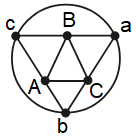
\includegraphics[width=2.5cm]{./img/octaedro.png} & &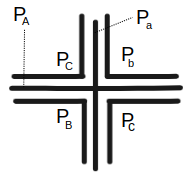
\includegraphics[width=4cm]{./img/representacaoOctaedro.png}  \\[\abovecaptionskip]
    \footnotesize \centering (a) O grafo octaedro $O_3$   & &  \footnotesize(b) Representação $B_1$-EPG do grafo $O_3$
  \end{tabular}

 \caption{O grafo octaedro $O_3$ e sua representação $B_1$-EPG}\label{fig:octaedro}
\end{figure}